193. \begin{figure}[ht!]
\center{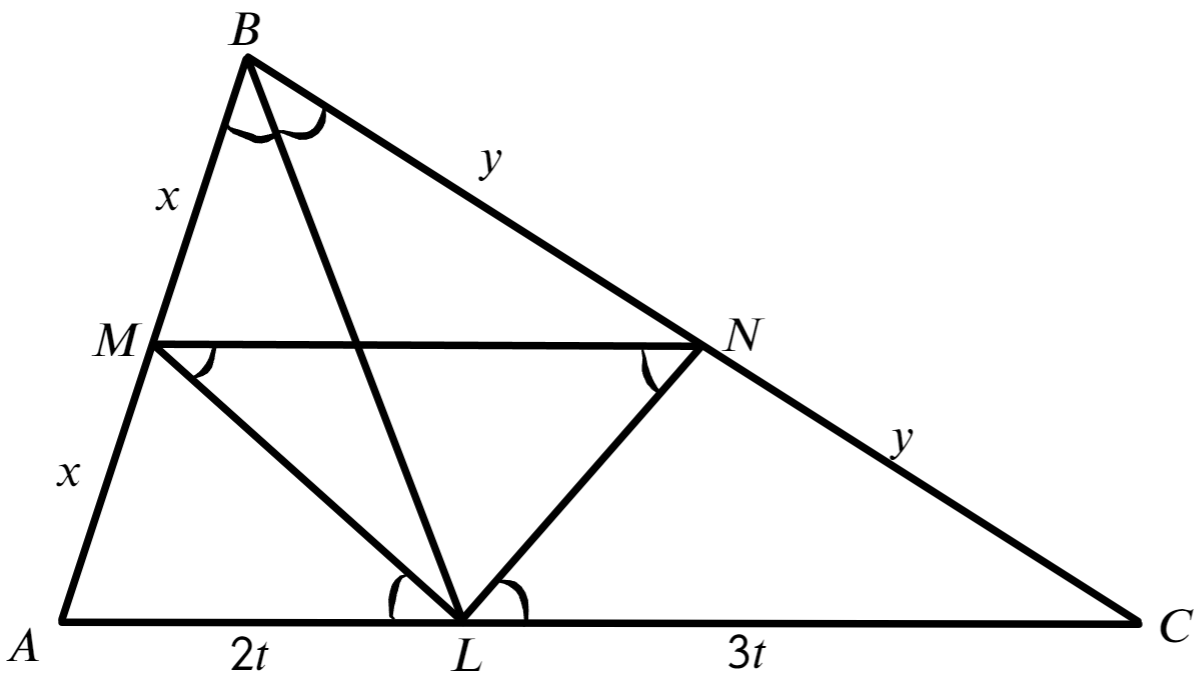
\includegraphics[scale=0.35]{g9-193.png}}
\end{figure}\\
Обозначим $AM=MB=x,\ CN=NB=y,\ AL=2t,\ LC=3t.$ Так как четырёхугольник $MBNL$ является вписанным, $\angle NML=\angle LBN=\angle LBM=\angle MNL.$ Так как $MN\parallel AC,$ из равенства накрест лежащих углов имеем соотношения $\angle ALM=\angle LMN=\angle MNL=\angle CLN.$ Треугольники $AML$ и $ALB$ подобны по двум углам ($\angle A$ --- общий, $\angle ALM=\angle ABL$), поэтому $\cfrac{AM}{AL}=\cfrac{AL}{AB},\ \cfrac{x}{2t}=\cfrac{2t}{x},\ 2x^2=4t^2,\ x=\sqrt{2}t.$ Аналогично $\cfrac{CN}{CL}=\cfrac{CL}{BC},\ \cfrac{y}{3t}=\cfrac{3t}{2y},\ 2y^2=9t^2,\ y=\cfrac{3}{\sqrt{2}}t.$ По теореме косинусов для треугольника $ABC$ получим равенство $(2x)^2+(2y)^2-2\cdot2x\cdot2y\cos(\angle B)=(5t)^2,\
8t^2+18t^2-24t^2\cos(\angle B)=25t^2,\ \cos(\angle B)=\cfrac{1}{24}.$ Окружность, описанная вокруг четырёхугольника $MBNL,$ описана также и вокруг треугольника $MBN,$ значит по теореме синусов имеем равенство $\cfrac{MN}{\sin(\angle B)}=16\sqrt{3},\ MN=16\sqrt{3}\cdot\sqrt{1-\cfrac{1}{576}}=\cfrac{10\sqrt{69}}{3}.$\\
